\section{Experiments and Results}
\label{sec:results}

\subsection{Baseline reproduction}

The tuned legacy msiPL reproduction obtained mean mSCF1 0.414 on GBM and 0.402
on CAC. These values lie inside the published aggregate intervals used for the
reproduction audit. S3PL was executable on both collections, but its GBM mean
remained below the reported paper result despite patch-size, normalisation,
format and mask checks. The CAC S3PL checkpoints were therefore re-evaluated at
the same section-specific peak counts as the VAE methods; no retraining was
needed. Matched S3PL averaged 0.5915 mSCF1.

\subsection{Does uniform context improve the VAE?}

On GBM, reconstruction MSE favoured uniform context in four sections and the
centre-only model in four (exact Wilcoxon $p=0.945$). Mean relative MSE change
was $-2.14\%$, but the median was $+0.52\%$ and one section strongly influenced
the mean. Uniform context used 130,751,056 parameters and approximately 2.90
GiB peak GPU memory, compared with 87,199,312 parameters and 2.05 GiB for the
centre-only model. \Cref{fig:recon} shows that local context did not provide a
consistent reconstruction advantage.

\begin{figure}[t]
  \centering
  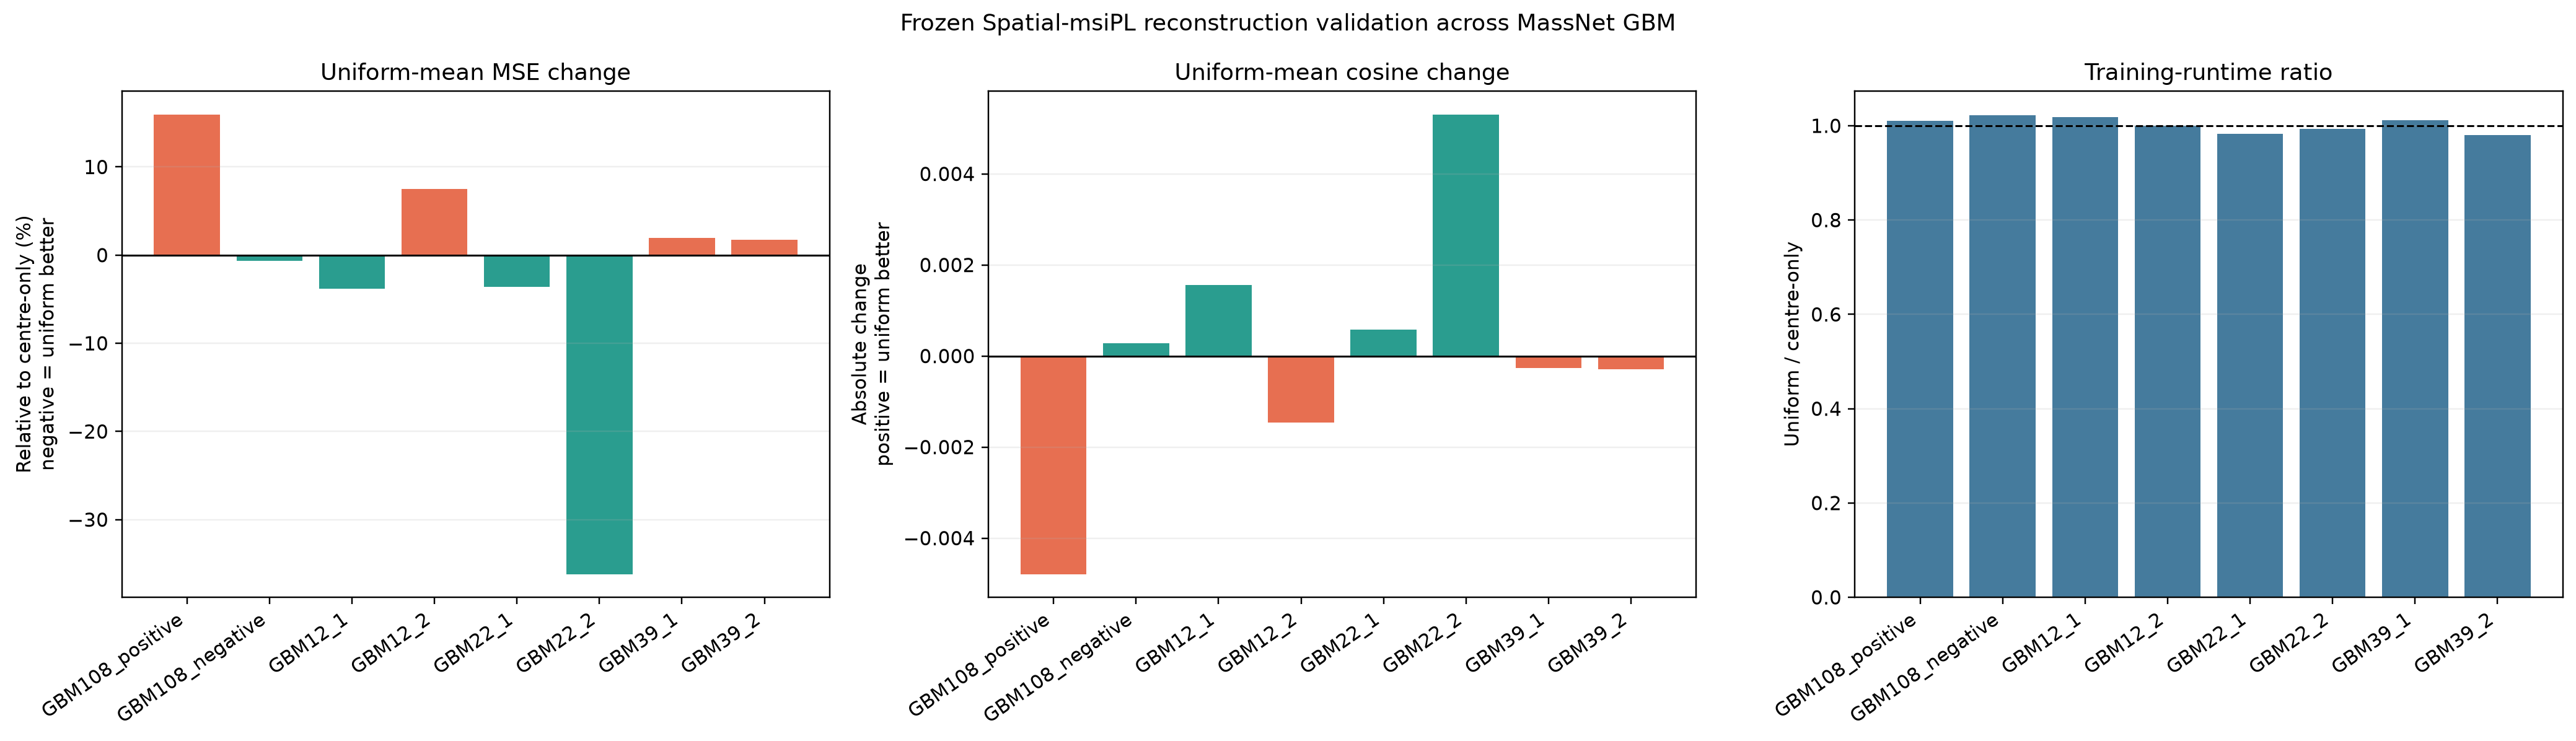
\includegraphics[width=\columnwidth]{images/gbm_reconstruction_validation.png}
  \caption{Paired whole-GBM reconstruction comparison. Negative MSE change
  favours uniform context; the heterogeneous section effects produce no
  consistent aggregate advantage.}
  \label{fig:recon}
\end{figure}

The peak-selection effect was also collection-dependent
(\Cref{fig:context}). On GBM, uniform-context IG averaged 0.4562 mSCF1 versus
0.4665 for centre-only IG, winning five of eight sections but with mean change
$-0.0103$. On CAC, it averaged 0.5595 versus 0.5285, won all eight sections and
had a mean paired gain of 0.0310 (exact $p=0.0078125$). Thus context changed the
nonlinear ranking beneficially on CAC without a corresponding universal gain
in reconstruction or GMM--mask agreement.

\begin{figure*}[t]
  \centering
  
\includegraphics[width=0.96\textwidth]{images/figure_2_context_effect_by_section.png}
  \caption{Section-wise change in mSCF1 from adding uniform neighbourhood
  context to the otherwise matched VAE and GMM-targeted IG procedure. Context
  is mixed on GBM but positive on every CAC section.}
  \label{fig:context}
\end{figure*}

\subsection{Does nonlinear attribution improve peak ranking?}

\Cref{fig:primary} summarises the primary matched-count result. On GBM,
centre-only IG and uniform-context IG averaged 0.4665 and 0.4562 mSCF1,
respectively, versus 0.3643 for legacy msiPL. At least one IG variant beat
legacy msiPL in every section; uniform-context IG alone did so in all eight
($p=0.0078125$). On CAC, centre-only and uniform-context IG averaged 0.5285 and
0.5595 versus 0.4024 for legacy msiPL; uniform-context IG again won all eight
paired sections ($p=0.0078125$).

\begin{figure*}[t]
  \centering
  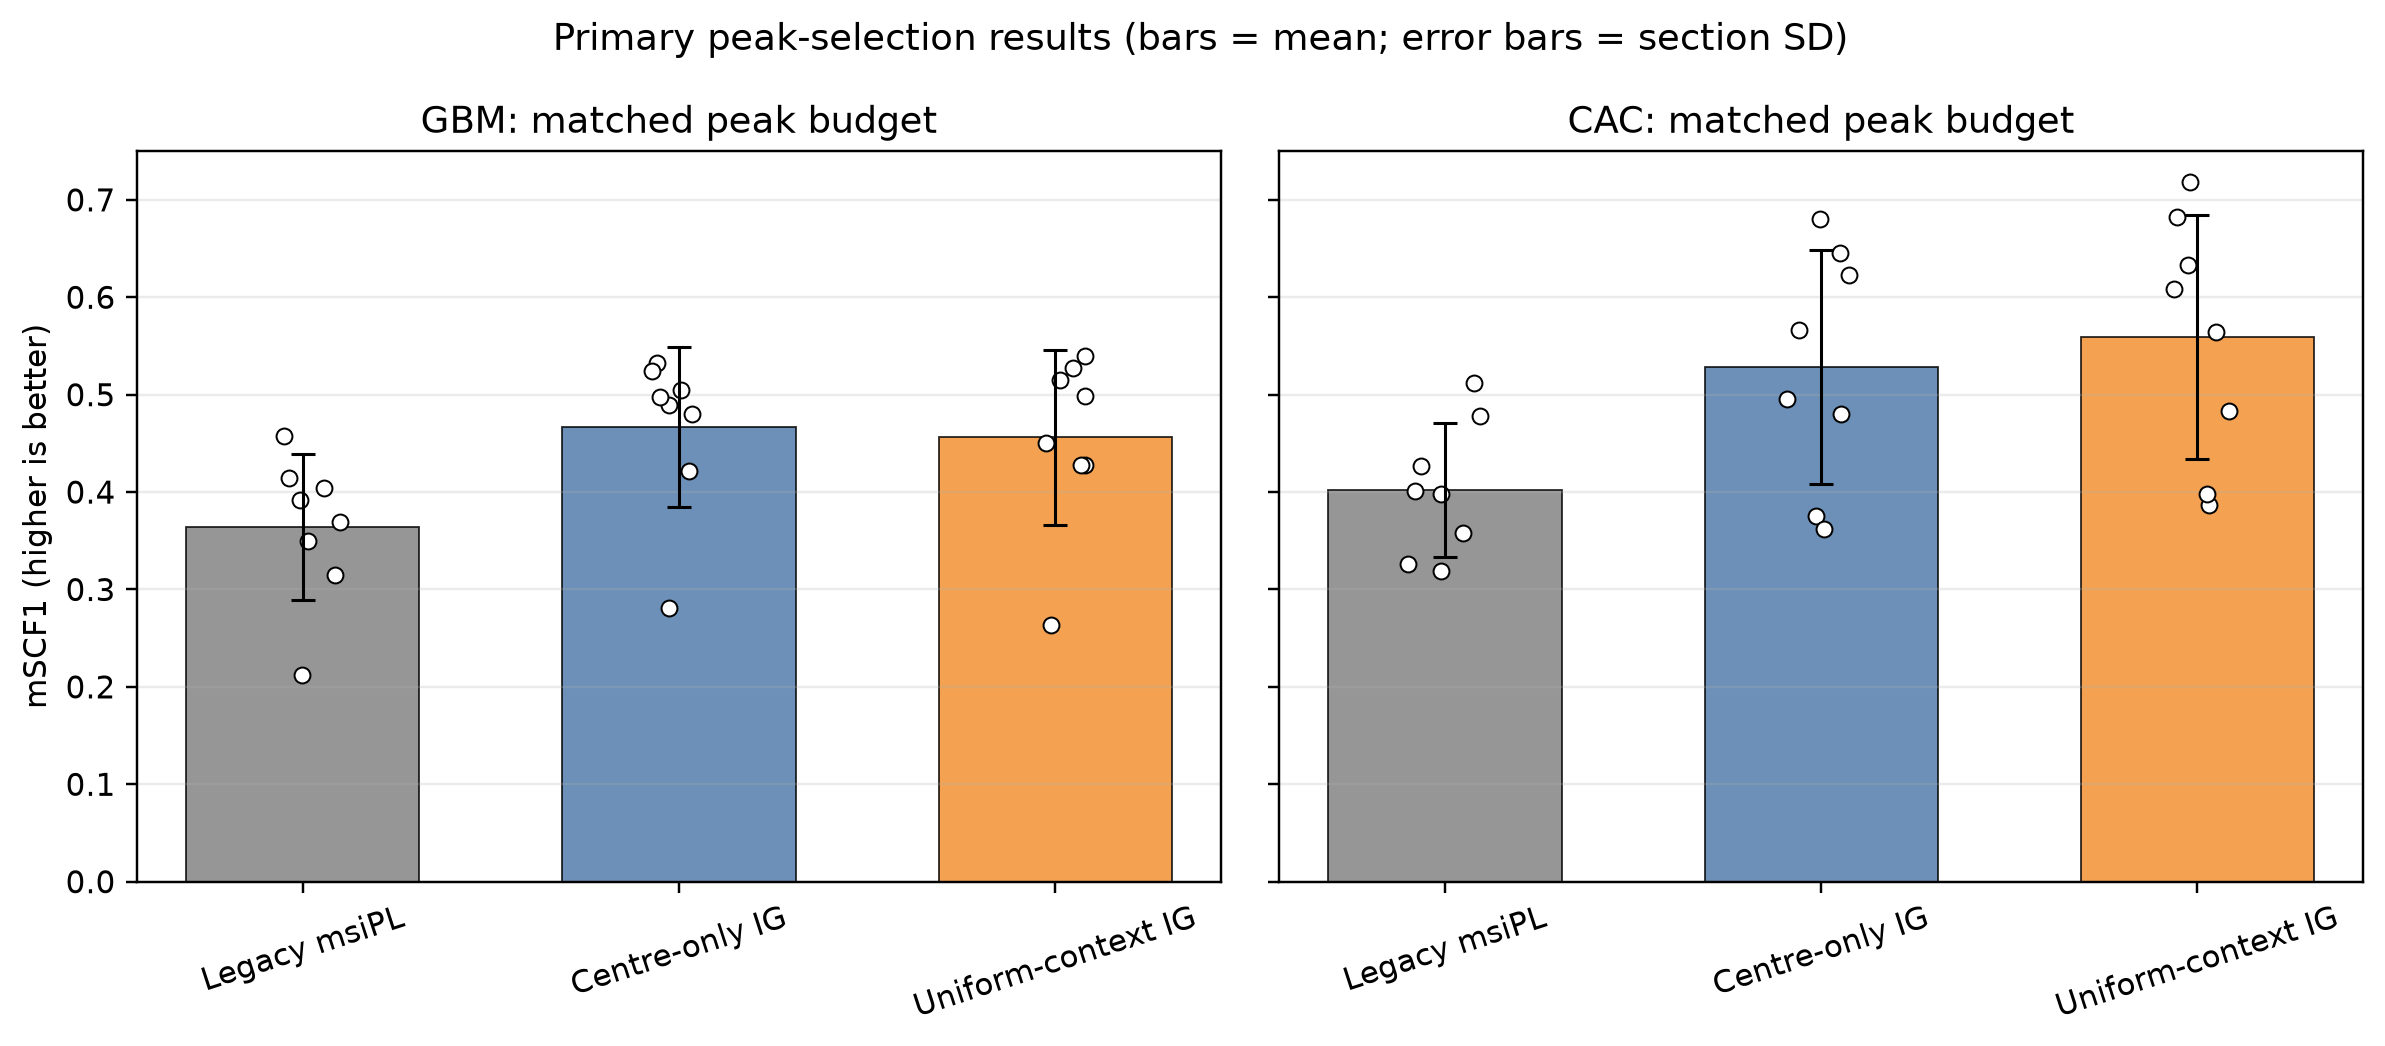
\includegraphics[width=0.96\textwidth]{images/figure_1_primary_peak_quality.png}
  \caption{Matched-count peak-selection quality across the two collections.
  Markers represent tissue sections; bars summarise method-level means. The
  consistent comparison is within collection and section, not between the two
  different datasets.}
  \label{fig:primary}
\end{figure*}

First-layer L2 was generally much weaker than nonlinear IG
(\Cref{fig:ablation}). On the initial GBM108-positive test at 530 peaks,
uniform-context IG achieved 0.528 mSCF1, legacy msiPL 0.404 and first-layer L2
0.068. IG passed the numerical completeness checks, and deleting IG-ranked
features caused a larger GMM-posterior drop than deleting L2-ranked or random
features. These results support the interpretation that gradients through the
complete nonlinear encoder and latent decision surface contain information that
is absent from the first layer alone.

\begin{figure}[t]
  \centering
  
\includegraphics[width=\columnwidth]{images/figure_3_explanation_ablation.png}
  \caption{Explanation-method ablation at matched peak counts. The simple
  first-layer L2 shortcut is not an adequate substitute for GMM-targeted
  nonlinear attribution.}
  \label{fig:ablation}
\end{figure}

S3PL remained stronger on matched CAC evaluation: 0.5915 versus 0.5595 for
uniform-context IG, winning six of eight sections (exact $p=0.0390625$). This
comparison establishes peak quality, but not equivalent computational
efficiency: S3PL used its released 10-epoch protocol whereas the VAE validation
used 100 epochs.

\subsection{Learned attention and training-seed stability}

Corrected attention, uniform mean and centre-only models were independently
trained with seeds 1--3 on the frozen GBM108-positive development section. Mean
mSCF1 was $0.5120\pm0.0179$, $0.5250\pm0.0132$ and
$0.5454\pm0.0188$ (sample standard deviation), respectively
(\Cref{fig:seeds}). Attention beat uniform mean in all three paired seeds, with
gains $+0.0347$, $+0.0120$ and $+0.0144$ (mean $+0.0204$). Mean GMM balanced
accuracy was 0.8745, 0.8735 and 0.8822.

\begin{figure*}[t]
  \centering
  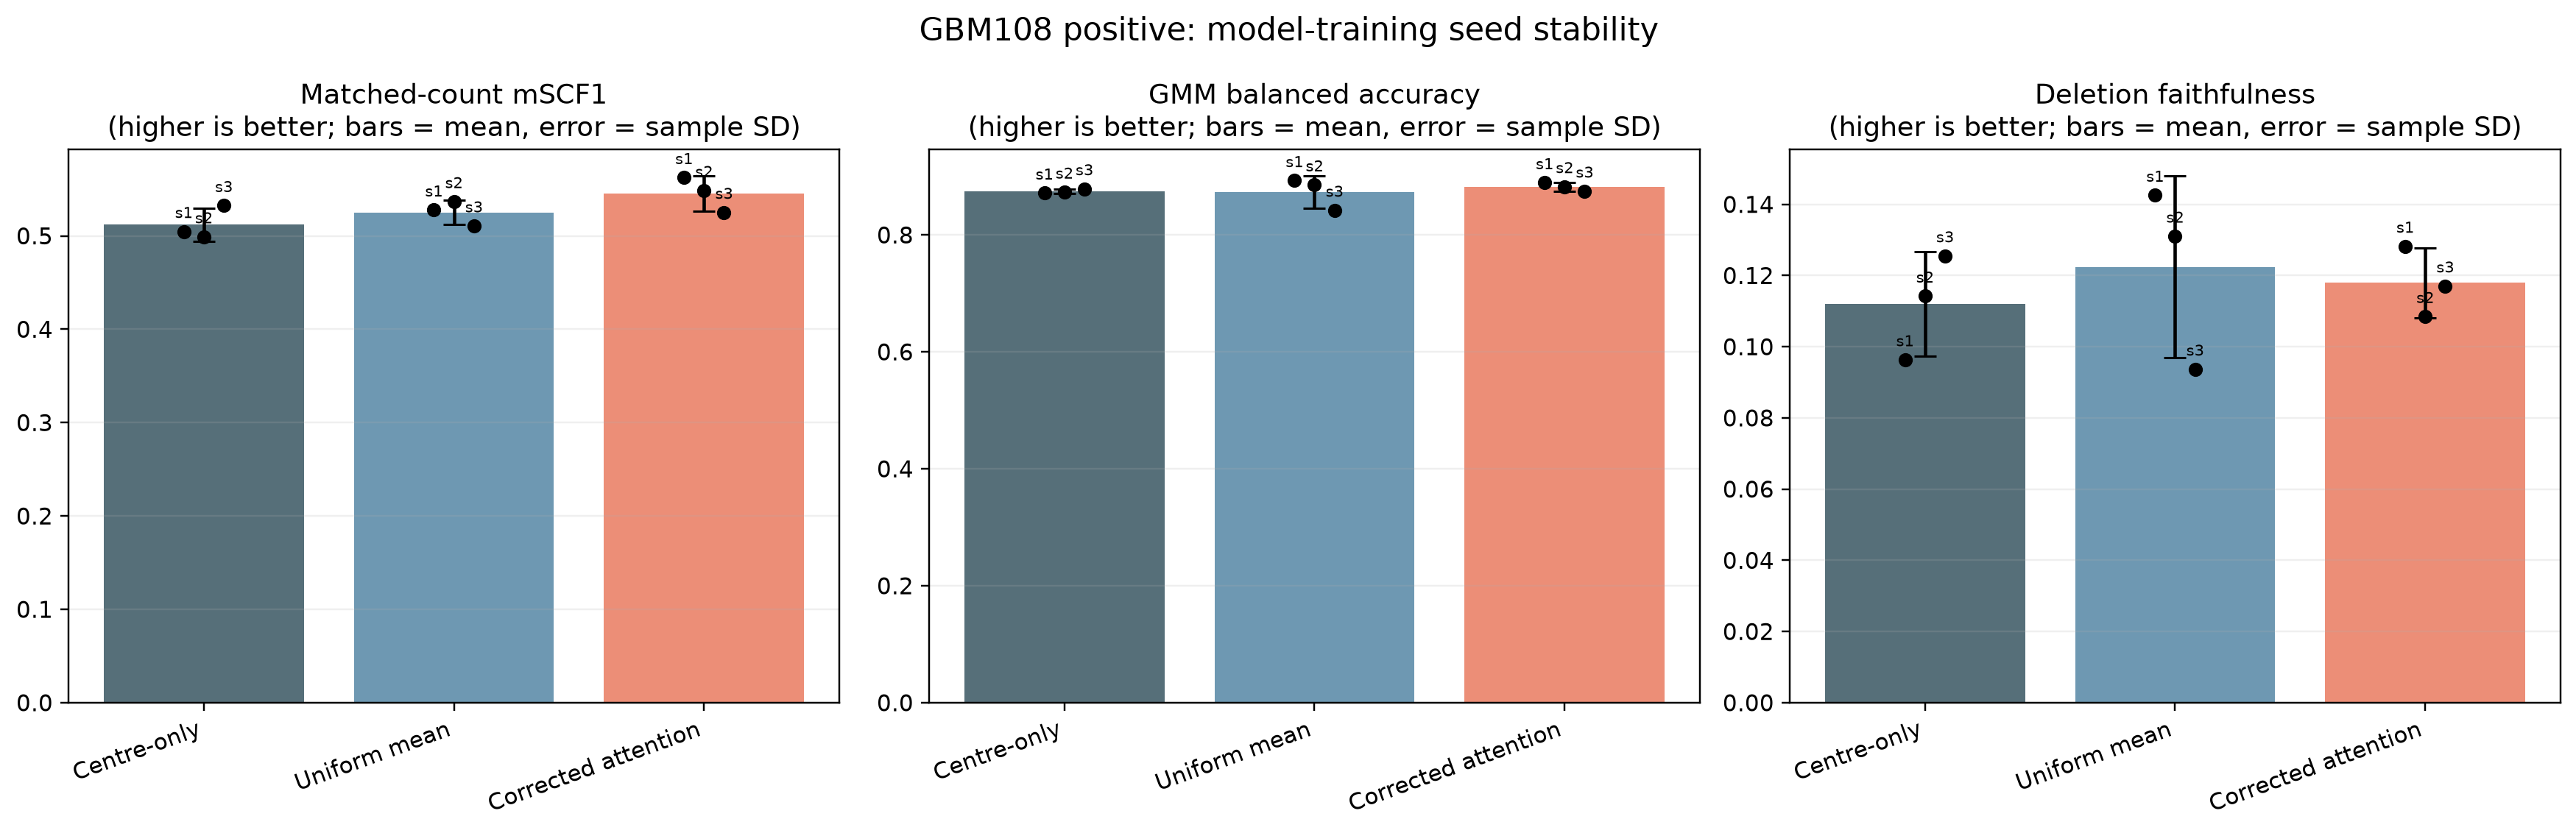
\includegraphics[width=0.95\textwidth]{images/figure_4_seed_stability.png}
  \caption{Targeted three-seed stability on GBM108-positive. Corrected
  attention improves matched-count mSCF1 over uniform averaging in every seed,
  but the experiment is restricted to one development section.}
  \label{fig:seeds}
\end{figure*}

The attention result did not pass the combined predeclared gate. Its mean
deletion-faithfulness score was 0.0045 below uniform mean and it won that metric
in only one seed. Peak allocated GPU memory also increased from about 2.90 GiB
for uniform mean to 3.20 GiB for attention. The result is therefore a stable
peak-quality improvement on one section, not evidence of a uniformly superior
model.
